\section{Results and Analysis}
\label{sec:results}
\subsection{General and Professional Decisions}
\begin{table}[t]
\centering
\footnotesize
\setlength{\tabcolsep}{4pt}
\caption{General-domain comparison. All local models use $T=1$; 2B results are preliminary.}
\label{tab:general}
\begin{tabular}{lrr}
\toprule
Model & ACC (\%) $\uparrow$ & ECE (\%) $\downarrow$ \\
\midrule
Qwen3.5-2B (imported) & 32.95 & 43.68 \\
Open-Jev & 52.33 & 10.54 \\
SemIF & 44.21 & 27.27 \\
Laya Multilingual & 40.22 & 23.04 \\
Jev & 68.35 & 11.45 \\
Chinese-Jev General & 69.20 & 3.78 \\
Ours 0.8B (step 10000) & 72.24 & 3.03 \\
Ours 2B (step 1000) & 70.55 & 4.58 \\
Ours 2B (step 2000) & 72.56 & 2.93 \\
\bottomrule
\end{tabular}
\par\vspace{3pt}\begin{minipage}{\columnwidth}\footnotesize Baseline rows are imported from Chinese-Jev~\citep{wang2026chinesejev}, not reproduced. The decision-fine-tuned 2B members differ from the imported Qwen baseline.\end{minipage}
\end{table}

Table~\ref{tab:general} compares general-domain performance. The completed 0.8B member reaches 72.24\% accuracy, 3.04 percentage points above the imported Chinese-Jev General result and 3.89 points above Jev. Its ECE is 3.03\%, compared with 3.78\% and 11.45\%, respectively. The preliminary 2B step-2000 checkpoint reaches 72.56\% accuracy and 2.93\% ECE. These comparisons describe the reported benchmark results; confidence intervals and a locally rerun baseline comparison are not available.

\begin{table*}[t]
\centering
\small
\setlength{\tabcolsep}{4pt}
\caption{Professional-domain comparison: accuracy / ECE (\%). Each local row uses one checkpoint for all domains; 2B snapshots are preliminary and uncalibrated.}
\label{tab:professional}
\begin{tabular}{lrrrrrrrr}
\toprule
& \multicolumn{2}{c}{Medical} & \multicolumn{2}{c}{Legal} & \multicolumn{2}{c}{Finance} & \multicolumn{2}{c}{Professional mean} \\ Model & ACC $\uparrow$ & ECE $\downarrow$ & ACC $\uparrow$ & ECE $\downarrow$ & ACC $\uparrow$ & ECE $\downarrow$ & ACC $\uparrow$ & ECE $\downarrow$ \\
\midrule
Qwen3.5-2B (imported) & 53.88 & 28.71 & 31.53 & 44.82 & 38.11 & 49.12 & 41.17 & 40.88 \\
Open-Jev & 73.08 & 2.88 & 44.07 & 23.15 & 48.11 & 10.19 & 55.09 & 12.07 \\
SemIF & 62.17 & 10.39 & 43.07 & 19.99 & 47.89 & 18.45 & 51.04 & 16.28 \\
Laya Multilingual & 24.55 & 43.05 & 34.72 & 31.49 & 38.31 & 26.18 & 32.53 & 33.57 \\
Jev & 84.29 & 5.70 & 68.35 & 8.03 & 78.39 & 2.98 & 77.01 & 5.57 \\
Chinese-Jev-S (3 models) & 87.65 & 7.25 & 60.10 & 17.45 & 64.72 & 11.55 & 70.82 & 12.08 \\
Ours 0.8B (single model) & 88.86 & 0.17 & 67.86 & 5.70 & 74.22 & 1.50 & 76.98 & 2.46 \\
Ours 2B (step 1000) & 87.69 & 0.67 & 55.67 & 6.83 & 66.94 & 3.63 & 70.10 & 3.71 \\
Ours 2B (step 2000) & 88.54 & 0.41 & 62.67 & 4.11 & 71.44 & 2.32 & 74.22 & 2.28 \\
\bottomrule
\end{tabular}
\par\vspace{3pt}\begin{minipage}{\textwidth}\footnotesize All baseline values are imported from Chinese-Jev~\citep{wang2026chinesejev}. The last baseline combines three specialist models. Means are unweighted across the three domains.\end{minipage}
\end{table*}

One 0.8B checkpoint covers all professional domains in Table~\ref{tab:professional}. It obtains 88.86\% medical, 67.86\% legal, and 74.22\% financial accuracy. Each exceeds the corresponding imported Chinese-Jev specialist result, by 1.21, 7.76, and 9.50 points. Its 76.98\% professional average is numerically close to Jev's 77.01\%, but this 0.03-point difference is not evidence of statistical equivalence. The model exceeds Jev in medicine, trails it by 0.49 points in law, and trails it by 4.17 points in finance.

The professional-domain average ECE is 2.46\% for 0.8B and 2.28\% for the 2B step-2000 snapshot. In the latter case, lower average ECE coexists with lower average accuracy (74.22\%). Accuracy and calibration therefore need to be examined jointly; neither is a substitute for the other.

\subsection{Aggregate and Typed Results}
\begin{table*}[t]
\centering
\small
\setlength{\tabcolsep}{4pt}
\caption{Full-benchmark aggregate results at $T=1$. Macro ACC averages four domains; score MAE is restricted to ordinal questions.}
\label{tab:aggregate}
\begin{tabular}{lrrrrrr}
\toprule
Model / checkpoint & Micro ACC (\%) & Macro ACC (\%) & ECE (\%) & NLL & Brier & Score MAE \\
\midrule
0.8B / step 10000 & 83.11 & 75.80 & 1.07 & 0.432 & 0.224 & 0.579 \\
2B / step 1000 & 81.55 & 70.22 & 2.03 & 0.493 & 0.248 & 0.612 \\
2B / step 2000 & 82.89 & 73.80 & 1.27 & 0.447 & 0.228 & 0.583 \\
\bottomrule
\end{tabular}
\end{table*}

Table~\ref{tab:aggregate} reports complementary aggregate metrics. The completed 0.8B model obtains 83.11\% micro accuracy and 75.80\% four-domain macro accuracy. The gap reflects the weight of the larger and easier medical subset. The 2B step-2000 snapshot obtains 82.89\% micro and 73.80\% macro accuracy, with distribution NLL 0.447 versus 0.432 for 0.8B.

\begin{table*}[t]
\centering
\small
\setlength{\tabcolsep}{4pt}
\caption{Question-type results at $T=1$. The 2B row group is preliminary. The total/hard counts identify the metric denominators.}
\label{tab:types}
\begin{tabular}{llrrrrr}
\toprule
Model / step & Type & Total / hard & ACC (\%) & ECE (\%) & NLL & Score MAE \\
\midrule
0.8B / 10000 & \texttt{noul} & 134,577 / 134,577 & 94.95 & 0.39 & 0.117 & -- \\
0.8B / 10000 & \texttt{choice} & 134,577 / 134,577 & 78.33 & 1.48 & 0.588 & -- \\
0.8B / 10000 & \texttt{score} & 38,746 / 35,668 & 56.47 & 2.35 & 0.987 & 0.579 \\
2B / 2000 & \texttt{noul} & 134,577 / 134,577 & 94.77 & 1.04 & 0.124 & -- \\
2B / 2000 & \texttt{choice} & 134,577 / 134,577 & 78.36 & 1.06 & 0.604 & -- \\
2B / 2000 & \texttt{score} & 38,746 / 35,668 & 55.18 & 3.04 & 1.024 & 0.583 \\
\bottomrule
\end{tabular}
\end{table*}

Question-type results in Table~\ref{tab:types} show that Boolean judgments are substantially easier than categorical and ordinal decisions in this benchmark. The 0.8B model reaches 94.95\% \noul{} accuracy, 78.33\% \choice{} accuracy, and 56.47\% hard-target \score{} accuracy. Its expected-score MAE is 0.579 level indices. The larger run is slightly higher on categorical accuracy at step 2000 (78.36\%), but lower on Boolean and ordinal accuracy. Because candidate counts, source tasks, and domain mixtures differ by type, these gaps should not be interpreted as controlled effects of interface design alone.

\subsection{Training Trajectories}
\begin{table*}[t]
\centering
\footnotesize
\setlength{\tabcolsep}{4pt}
\caption{Checkpoint trajectory for the 0.8B cross-entropy run. All test results are full-benchmark, uncalibrated measurements.}
\label{tab:trajectory}
\begin{tabular}{rrrrrrrrr}
\toprule
Step & Val. NLL & General ACC & Medical ACC & Legal ACC & Finance ACC & Prof. ACC & Prof. ECE & Micro ECE \\
\midrule
2,000 & 0.739 & 69.04 & 86.78 & 54.07 & 64.17 & 68.34 & 2.73 & 1.63 \\
3,000 & 0.691 & 70.26 & 87.22 & 58.93 & 68.67 & 71.61 & 1.75 & 1.25 \\
5,000 & 0.676 & 70.90 & 87.89 & 63.37 & 71.17 & 74.14 & 1.49 & 0.84 \\
10,000 & 0.600 & 72.24 & 88.86 & 67.86 & 74.22 & 76.98 & 2.46 & 1.07 \\
\bottomrule
\end{tabular}
\par\vspace{3pt}\begin{minipage}{\textwidth}\footnotesize Accuracy and ECE are percentages. Checkpoints are selected using validation distribution NLL, not these test metrics.\end{minipage}
\end{table*}

\begin{figure*}[t]
\centering
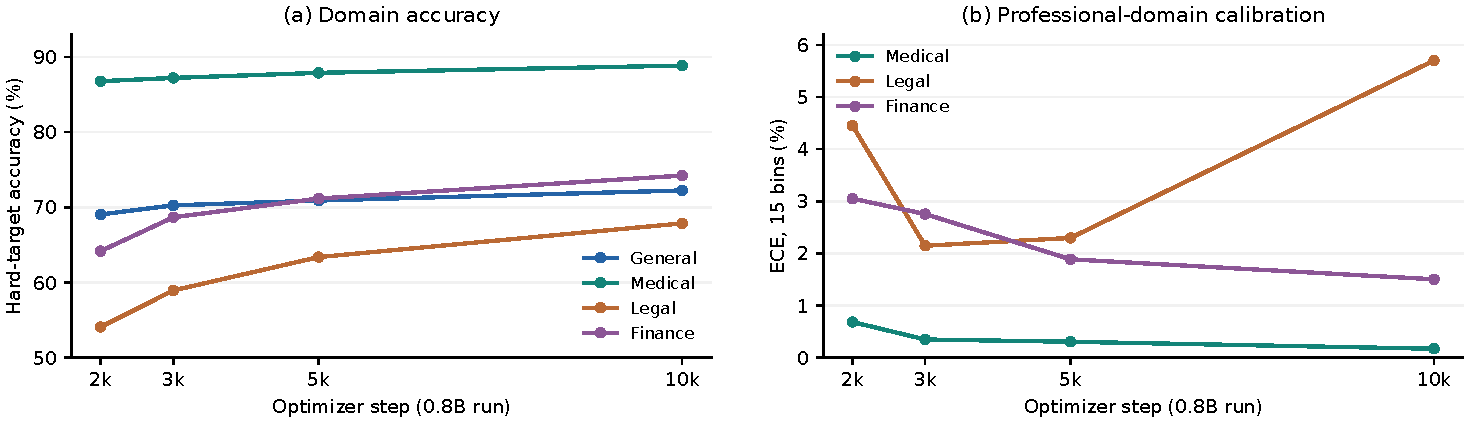
\includegraphics[width=\textwidth]{figures/trajectory.pdf}
\caption{Checkpoints from the same 0.8B cross-entropy run. Left: accuracy improves across all four domains. Right: professional-domain ECE does not improve monotonically; the legal subset worsens late in training. All points use full CJ-Bench evaluation at $T=1$. Lines connect measured checkpoints and do not represent independent training replicates.}
\label{fig:trajectory}
\end{figure*}
Across the four validation-selected 0.8B checkpoints in Table~\ref{tab:trajectory} and Figure~\ref{fig:trajectory}, validation distribution NLL falls from 0.739 to 0.600. Legal accuracy rises from 54.07\% to 67.86\%, finance from 64.17\% to 74.22\%, general from 69.04\% to 72.24\%, and medicine from 86.78\% to 88.86\%. The strongest gains are in the two domains with the least training data, although this observation alone does not establish the mechanism of transfer.

Calibration is non-monotonic. The professional average ECE is 2.73\%, 1.75\%, 1.49\%, and 2.46\% at steps 2000, 3000, 5000, and 10000. Legal ECE rises from 2.30\% at step 5000 to 5.70\% at step 10000 even as legal accuracy improves. Choosing the checkpoint with the best test ECE would conflict with the stated selection protocol; the released checkpoint remains the one selected by validation NLL.

\subsection{What the 2B Snapshots Establish}
The 2B run improves across both available full evaluations. Between steps 1000 and 2000, general accuracy rises from 70.55\% to 72.56\%, medicine from 87.69\% to 88.54\%, law from 55.67\% to 62.67\%, and finance from 66.94\% to 71.44\%. The professional average rises from 70.10\% to 74.22\%, and micro ECE falls from 2.03\% to 1.27\%.

At 40.13\% of the planned epoch, 2B has a higher general-domain point estimate than the completed 0.8B run by 0.31 points, but is lower in the other three domains. Neither completion quality nor monotonic gains with scale can be inferred. Size, training objective, minimum batch, token budget, and consumed data all differ. In particular, there is no matched 2B cross-entropy-only run here that would isolate RLCD, and no completed 2B result that would isolate training completion. We use ``family'' to denote a common model interface and adaptation pipeline across the two instantiated sizes, not a demonstrated scaling law.
